% ASTER figures for a two-column manuscript.
% Add to the preamble:
%   \usepackage{graphicx}
%   \usepackage{amsmath,amssymb}
%   \graphicspath{{docs/ASTER/figures/}}
% Then, when compiling from the repository root, use:
%   % ASTER figures for a two-column manuscript.
% Add to the preamble:
%   \usepackage{graphicx}
%   \usepackage{amsmath,amssymb}
%   \graphicspath{{docs/ASTER/figures/}}
% Then, when compiling from the repository root, use:
%   % ASTER figures for a two-column manuscript.
% Add to the preamble:
%   \usepackage{graphicx}
%   \usepackage{amsmath,amssymb}
%   \graphicspath{{docs/ASTER/figures/}}
% Then, when compiling from the repository root, use:
%   % ASTER figures for a two-column manuscript.
% Add to the preamble:
%   \usepackage{graphicx}
%   \usepackage{amsmath,amssymb}
%   \graphicspath{{docs/ASTER/figures/}}
% Then, when compiling from the repository root, use:
%   \input{docs/ASTER/figures/figures.tex}
% Paths are relative to the LaTeX compilation directory. If compiling from a
% paper/ subdirectory, use ../docs/ASTER/figures/ in both paths instead.
% Each source PDF is 7.0 inches wide. The template's \textwidth determines the
% final scale; inspect text at that scale in the final manuscript PDF.
% The English captions are mirrored in captions.en.md.

\begin{figure*}[t]
  \centering
  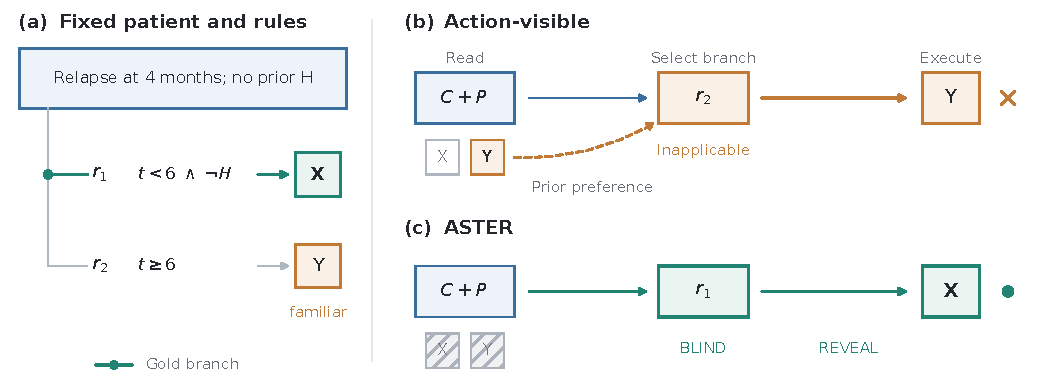
\includegraphics[width=\textwidth]{fig01_tlbs.pdf}
  \caption{\textbf{Treatment-led branch selection as a testable failure mode.} (a) In this fictional action-swap (SW) example, the patient relapses at $t=4$ months with no prior H. The supplied rules make $r_1:(t<6\land\neg H)\to X$ applicable and $r_2:(t\ge6)\to Y$ inapplicable. (b) The action-visible route illustrates the hypothesis that a preference for familiar Y can redirect selection toward its sibling branch. (c) ASTER is designed to select $r_1$ before revealing X. Both routes retain the same patient facts, conditions, and X/Y tokens; only the selection-stage attention mask changes. The dashed arrow and displayed outcomes are schematic, not observed model traces.}
  \label{fig:aster-tlbs}
\end{figure*}

\begin{figure*}[t]
  \centering
  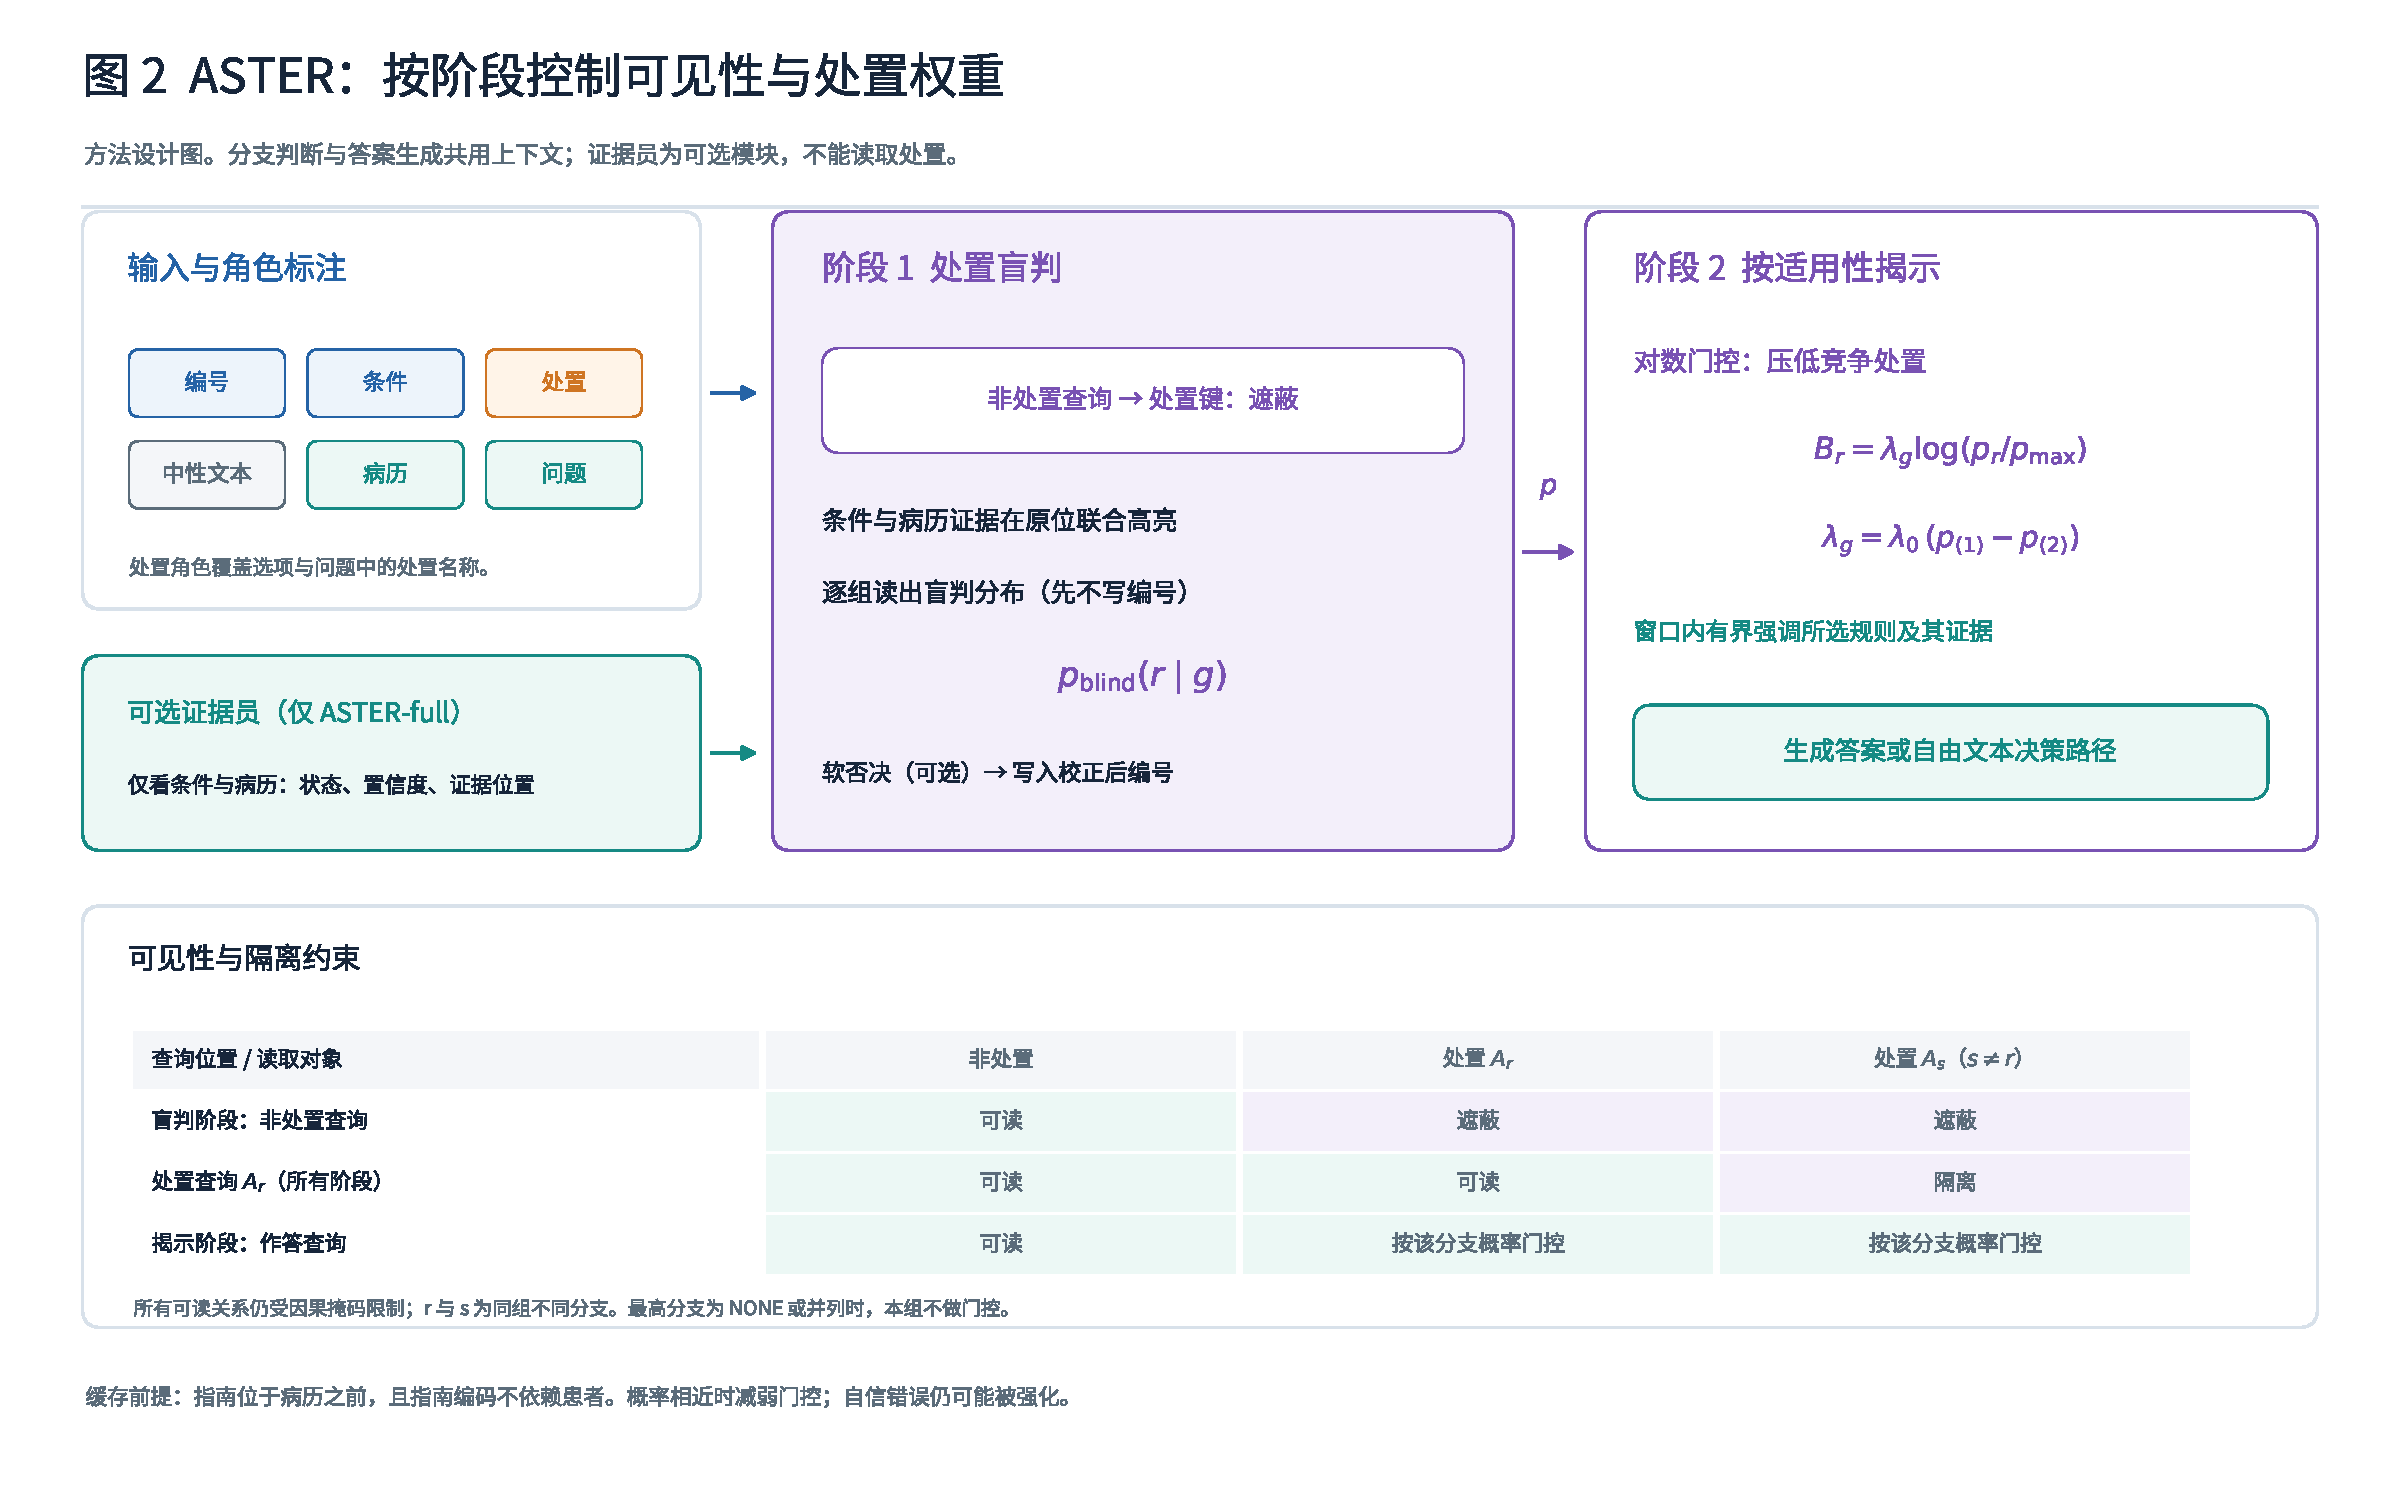
\includegraphics[width=\textwidth]{fig02_aster.pdf}
  \caption{\textbf{ASTER operators in a shared full context.} (a) The matrix shows representative-token query-key masks combined with causal masking. All BLIND non-action queries, including omitted neutral N and question Q positions, are blocked from action keys. Action mentions in questions/options retain the act role. The black outline marks cross-fragment action isolation, maintained in both phases. B is a fixed non-action readout position before branch-ID writing. (b) The optional clerk reads conditions C and patient text P and returns atomic states, confidence, and evidence. ASTER-full jointly highlights condition/evidence spans $(C,E)$ for post-prefix queries and applies a soft veto to obtain $p$ from $p_{\mathrm{blind}}$, both including NONE. This is joint highlighting, not pairwise binding. The adjusted distribution determines the written ID and both REVEAL controls. (c) For $p_1>\max(p_2,p_{\mathrm{NONE}})$, gating adds $b_r=\lambda_g\log(p_r/p_{\max})$ to rule-action keys across all layers/heads; emphasis adds bounded $\beta$ to selected rule/evidence tokens within specified layers when $p_{\max}\ge\tau$. Ties or a top NONE disable both controls. Purple elements are ASTER-full only. Only a fixed, patient-independent guideline prefix is cached; patient-dependent operations follow it.}
  \label{fig:aster-method}
\end{figure*}

\begin{figure*}[t]
  \centering
  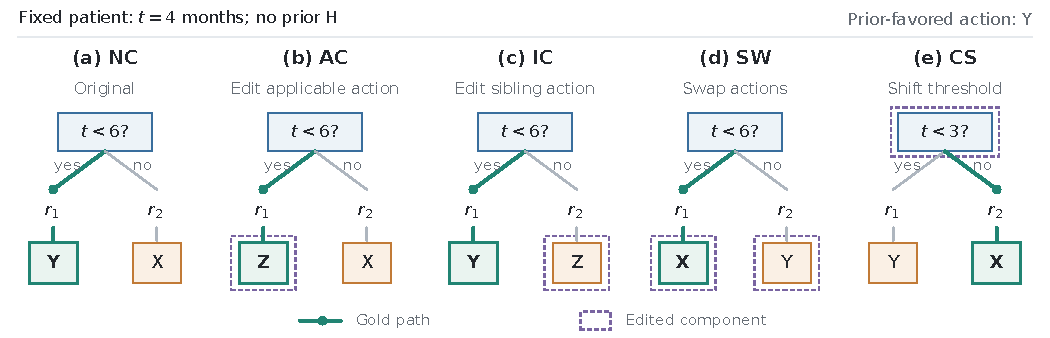
\includegraphics[width=\textwidth]{fig03_protocol.pdf}
  \caption{\textbf{Five paired guideline variants for a fixed fictional patient.} Each panel uses $t=4$ months and no prior H. NC retains the original rules; AC replaces the applicable action; IC replaces only the sibling action; SW exchanges the two actions; and CS shifts the threshold from 6 to 3 months, changing the applicable branch. The gold routes are $r_1\to Y$, $r_1\to Z$, $r_1\to Y$, $r_1\to X$, and $r_2\to X$, respectively. Identical tree layouts expose the local intervention: dashed outlines mark edited components, and the emphasized path marks the gold route. The common no-H condition is omitted from the miniature trees. Y is stipulated to be prior-favored in this illustration. SW reproduces the task in Figure 1; no model predictions are shown.}
  \label{fig:aster-protocol}
\end{figure*}

\begin{figure*}[t]
  \centering
  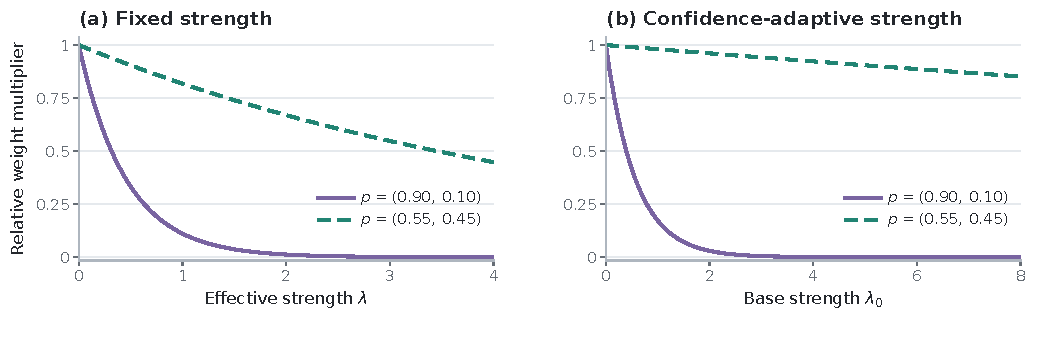
\includegraphics[width=\textwidth]{fig04_gate.pdf}
  \caption{\textbf{Analytic effect of the logarithmic action gate.} For fixed branch probabilities, pre-gate attention scores, and other biases, the gate multiplies the competing-to-top action-weight ratio by $m=(p_{\mathrm{comp}}/p_{\mathrm{top}})^\lambda$. (a) The effective strength $\lambda$ is varied directly. (b) The base strength $\lambda_0$ is varied with $\lambda=\lambda_0(p_{\mathrm{top}}-p_{\mathrm{comp}})$. Curves use the declared two-rule distributions $(0.90,0.10)$ and $(0.55,0.45)$, with zero NONE mass. They are exact formula evaluations, not measured attention probabilities, accuracy, or robustness. The plotted quantity is a relative multiplier on unnormalized attention weight, rather than the selected branch's share of total attention.}
  \label{fig:aster-gate}
\end{figure*}


% Paths are relative to the LaTeX compilation directory. If compiling from a
% paper/ subdirectory, use ../docs/ASTER/figures/ in both paths instead.
% Each source PDF is 7.0 inches wide. The template's \textwidth determines the
% final scale; inspect text at that scale in the final manuscript PDF.
% The English captions are mirrored in captions.en.md.

\begin{figure*}[t]
  \centering
  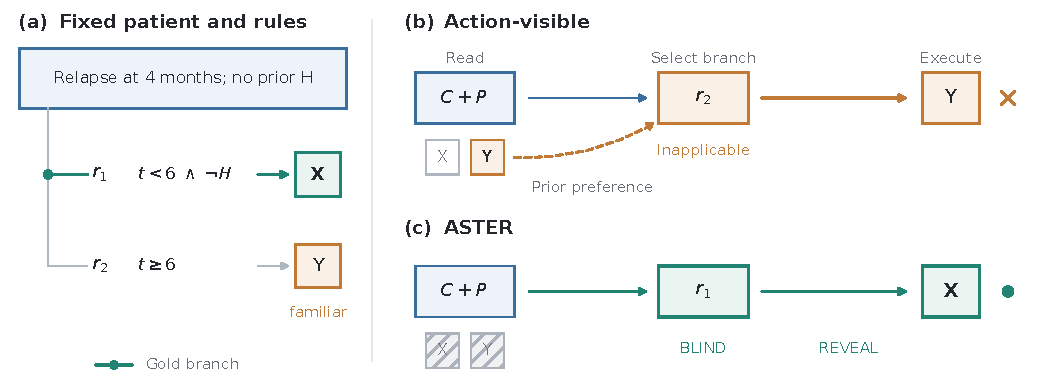
\includegraphics[width=\textwidth]{fig01_tlbs.pdf}
  \caption{\textbf{Treatment-led branch selection as a testable failure mode.} (a) In this fictional action-swap (SW) example, the patient relapses at $t=4$ months with no prior H. The supplied rules make $r_1:(t<6\land\neg H)\to X$ applicable and $r_2:(t\ge6)\to Y$ inapplicable. (b) The action-visible route illustrates the hypothesis that a preference for familiar Y can redirect selection toward its sibling branch. (c) ASTER is designed to select $r_1$ before revealing X. Both routes retain the same patient facts, conditions, and X/Y tokens; only the selection-stage attention mask changes. The dashed arrow and displayed outcomes are schematic, not observed model traces.}
  \label{fig:aster-tlbs}
\end{figure*}

\begin{figure*}[t]
  \centering
  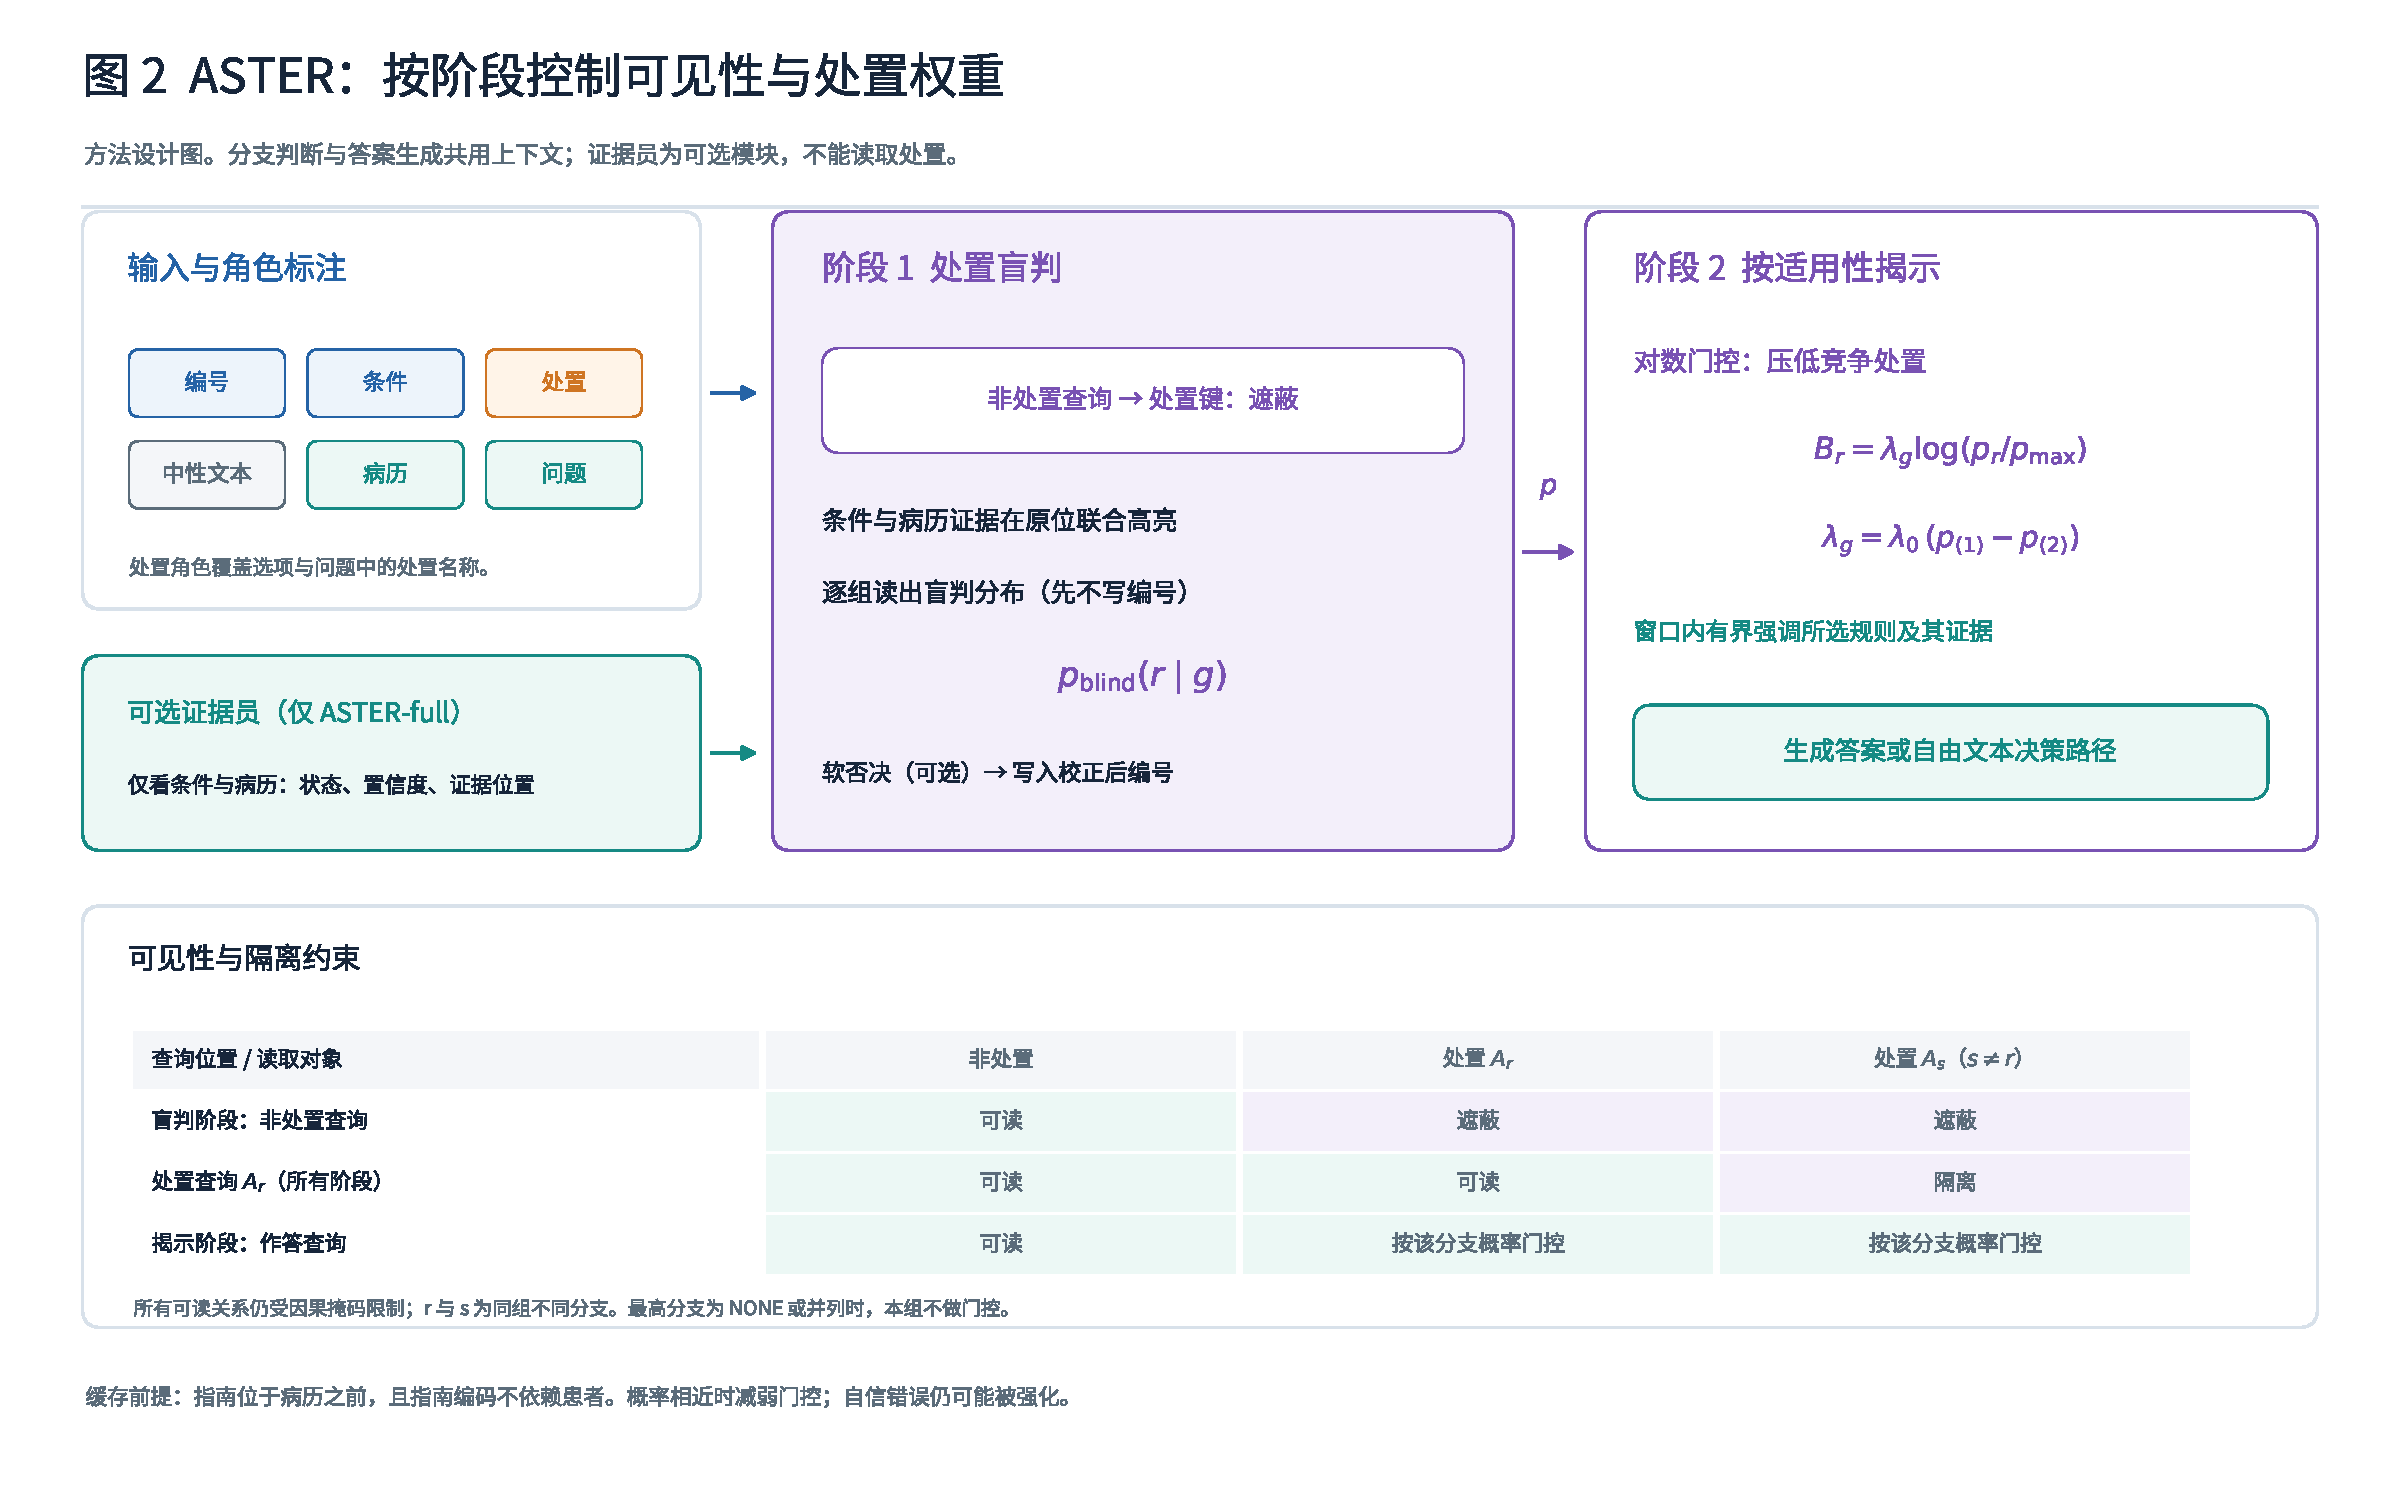
\includegraphics[width=\textwidth]{fig02_aster.pdf}
  \caption{\textbf{ASTER operators in a shared full context.} (a) The matrix shows representative-token query-key masks combined with causal masking. All BLIND non-action queries, including omitted neutral N and question Q positions, are blocked from action keys. Action mentions in questions/options retain the act role. The black outline marks cross-fragment action isolation, maintained in both phases. B is a fixed non-action readout position before branch-ID writing. (b) The optional clerk reads conditions C and patient text P and returns atomic states, confidence, and evidence. ASTER-full jointly highlights condition/evidence spans $(C,E)$ for post-prefix queries and applies a soft veto to obtain $p$ from $p_{\mathrm{blind}}$, both including NONE. This is joint highlighting, not pairwise binding. The adjusted distribution determines the written ID and both REVEAL controls. (c) For $p_1>\max(p_2,p_{\mathrm{NONE}})$, gating adds $b_r=\lambda_g\log(p_r/p_{\max})$ to rule-action keys across all layers/heads; emphasis adds bounded $\beta$ to selected rule/evidence tokens within specified layers when $p_{\max}\ge\tau$. Ties or a top NONE disable both controls. Purple elements are ASTER-full only. Only a fixed, patient-independent guideline prefix is cached; patient-dependent operations follow it.}
  \label{fig:aster-method}
\end{figure*}

\begin{figure*}[t]
  \centering
  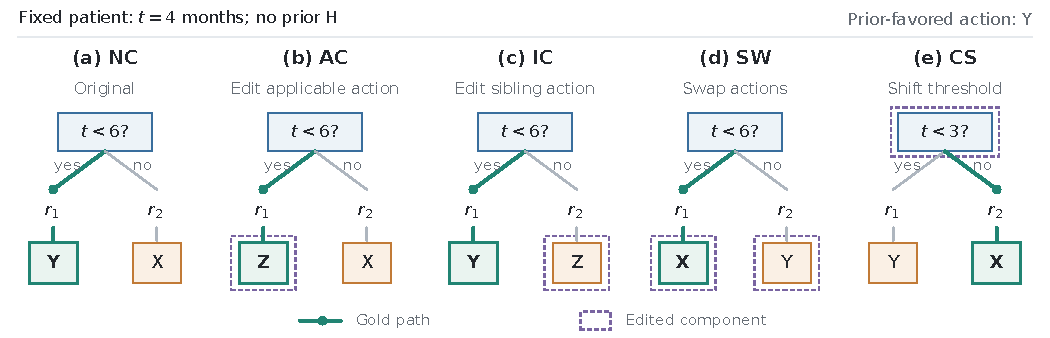
\includegraphics[width=\textwidth]{fig03_protocol.pdf}
  \caption{\textbf{Five paired guideline variants for a fixed fictional patient.} Each panel uses $t=4$ months and no prior H. NC retains the original rules; AC replaces the applicable action; IC replaces only the sibling action; SW exchanges the two actions; and CS shifts the threshold from 6 to 3 months, changing the applicable branch. The gold routes are $r_1\to Y$, $r_1\to Z$, $r_1\to Y$, $r_1\to X$, and $r_2\to X$, respectively. Identical tree layouts expose the local intervention: dashed outlines mark edited components, and the emphasized path marks the gold route. The common no-H condition is omitted from the miniature trees. Y is stipulated to be prior-favored in this illustration. SW reproduces the task in Figure 1; no model predictions are shown.}
  \label{fig:aster-protocol}
\end{figure*}

\begin{figure*}[t]
  \centering
  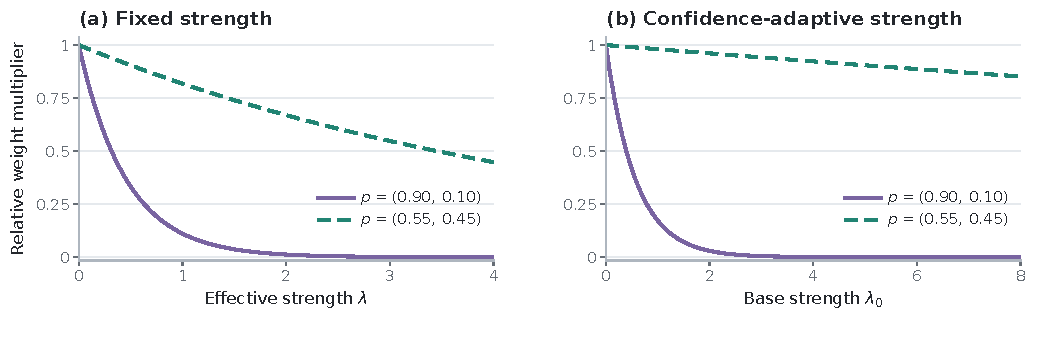
\includegraphics[width=\textwidth]{fig04_gate.pdf}
  \caption{\textbf{Analytic effect of the logarithmic action gate.} For fixed branch probabilities, pre-gate attention scores, and other biases, the gate multiplies the competing-to-top action-weight ratio by $m=(p_{\mathrm{comp}}/p_{\mathrm{top}})^\lambda$. (a) The effective strength $\lambda$ is varied directly. (b) The base strength $\lambda_0$ is varied with $\lambda=\lambda_0(p_{\mathrm{top}}-p_{\mathrm{comp}})$. Curves use the declared two-rule distributions $(0.90,0.10)$ and $(0.55,0.45)$, with zero NONE mass. They are exact formula evaluations, not measured attention probabilities, accuracy, or robustness. The plotted quantity is a relative multiplier on unnormalized attention weight, rather than the selected branch's share of total attention.}
  \label{fig:aster-gate}
\end{figure*}


% Paths are relative to the LaTeX compilation directory. If compiling from a
% paper/ subdirectory, use ../docs/ASTER/figures/ in both paths instead.
% Each source PDF is 7.0 inches wide. The template's \textwidth determines the
% final scale; inspect text at that scale in the final manuscript PDF.
% The English captions are mirrored in captions.en.md.

\begin{figure*}[t]
  \centering
  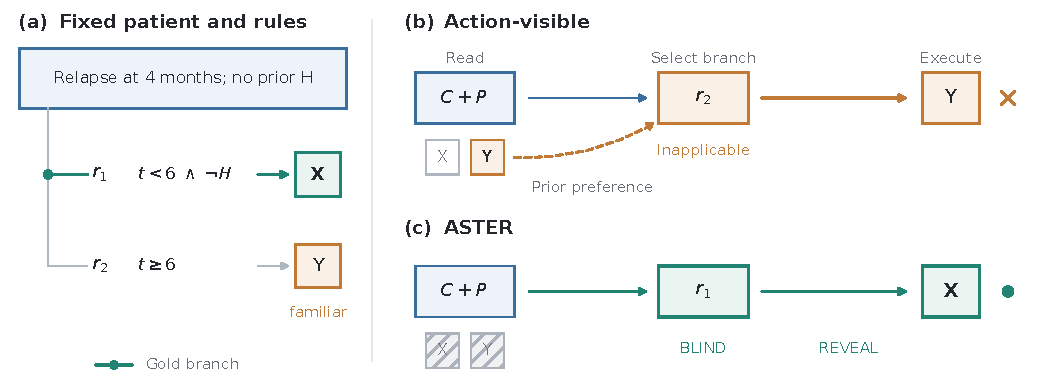
\includegraphics[width=\textwidth]{fig01_tlbs.pdf}
  \caption{\textbf{Treatment-led branch selection as a testable failure mode.} (a) In this fictional action-swap (SW) example, the patient relapses at $t=4$ months with no prior H. The supplied rules make $r_1:(t<6\land\neg H)\to X$ applicable and $r_2:(t\ge6)\to Y$ inapplicable. (b) The action-visible route illustrates the hypothesis that a preference for familiar Y can redirect selection toward its sibling branch. (c) ASTER is designed to select $r_1$ before revealing X. Both routes retain the same patient facts, conditions, and X/Y tokens; only the selection-stage attention mask changes. The dashed arrow and displayed outcomes are schematic, not observed model traces.}
  \label{fig:aster-tlbs}
\end{figure*}

\begin{figure*}[t]
  \centering
  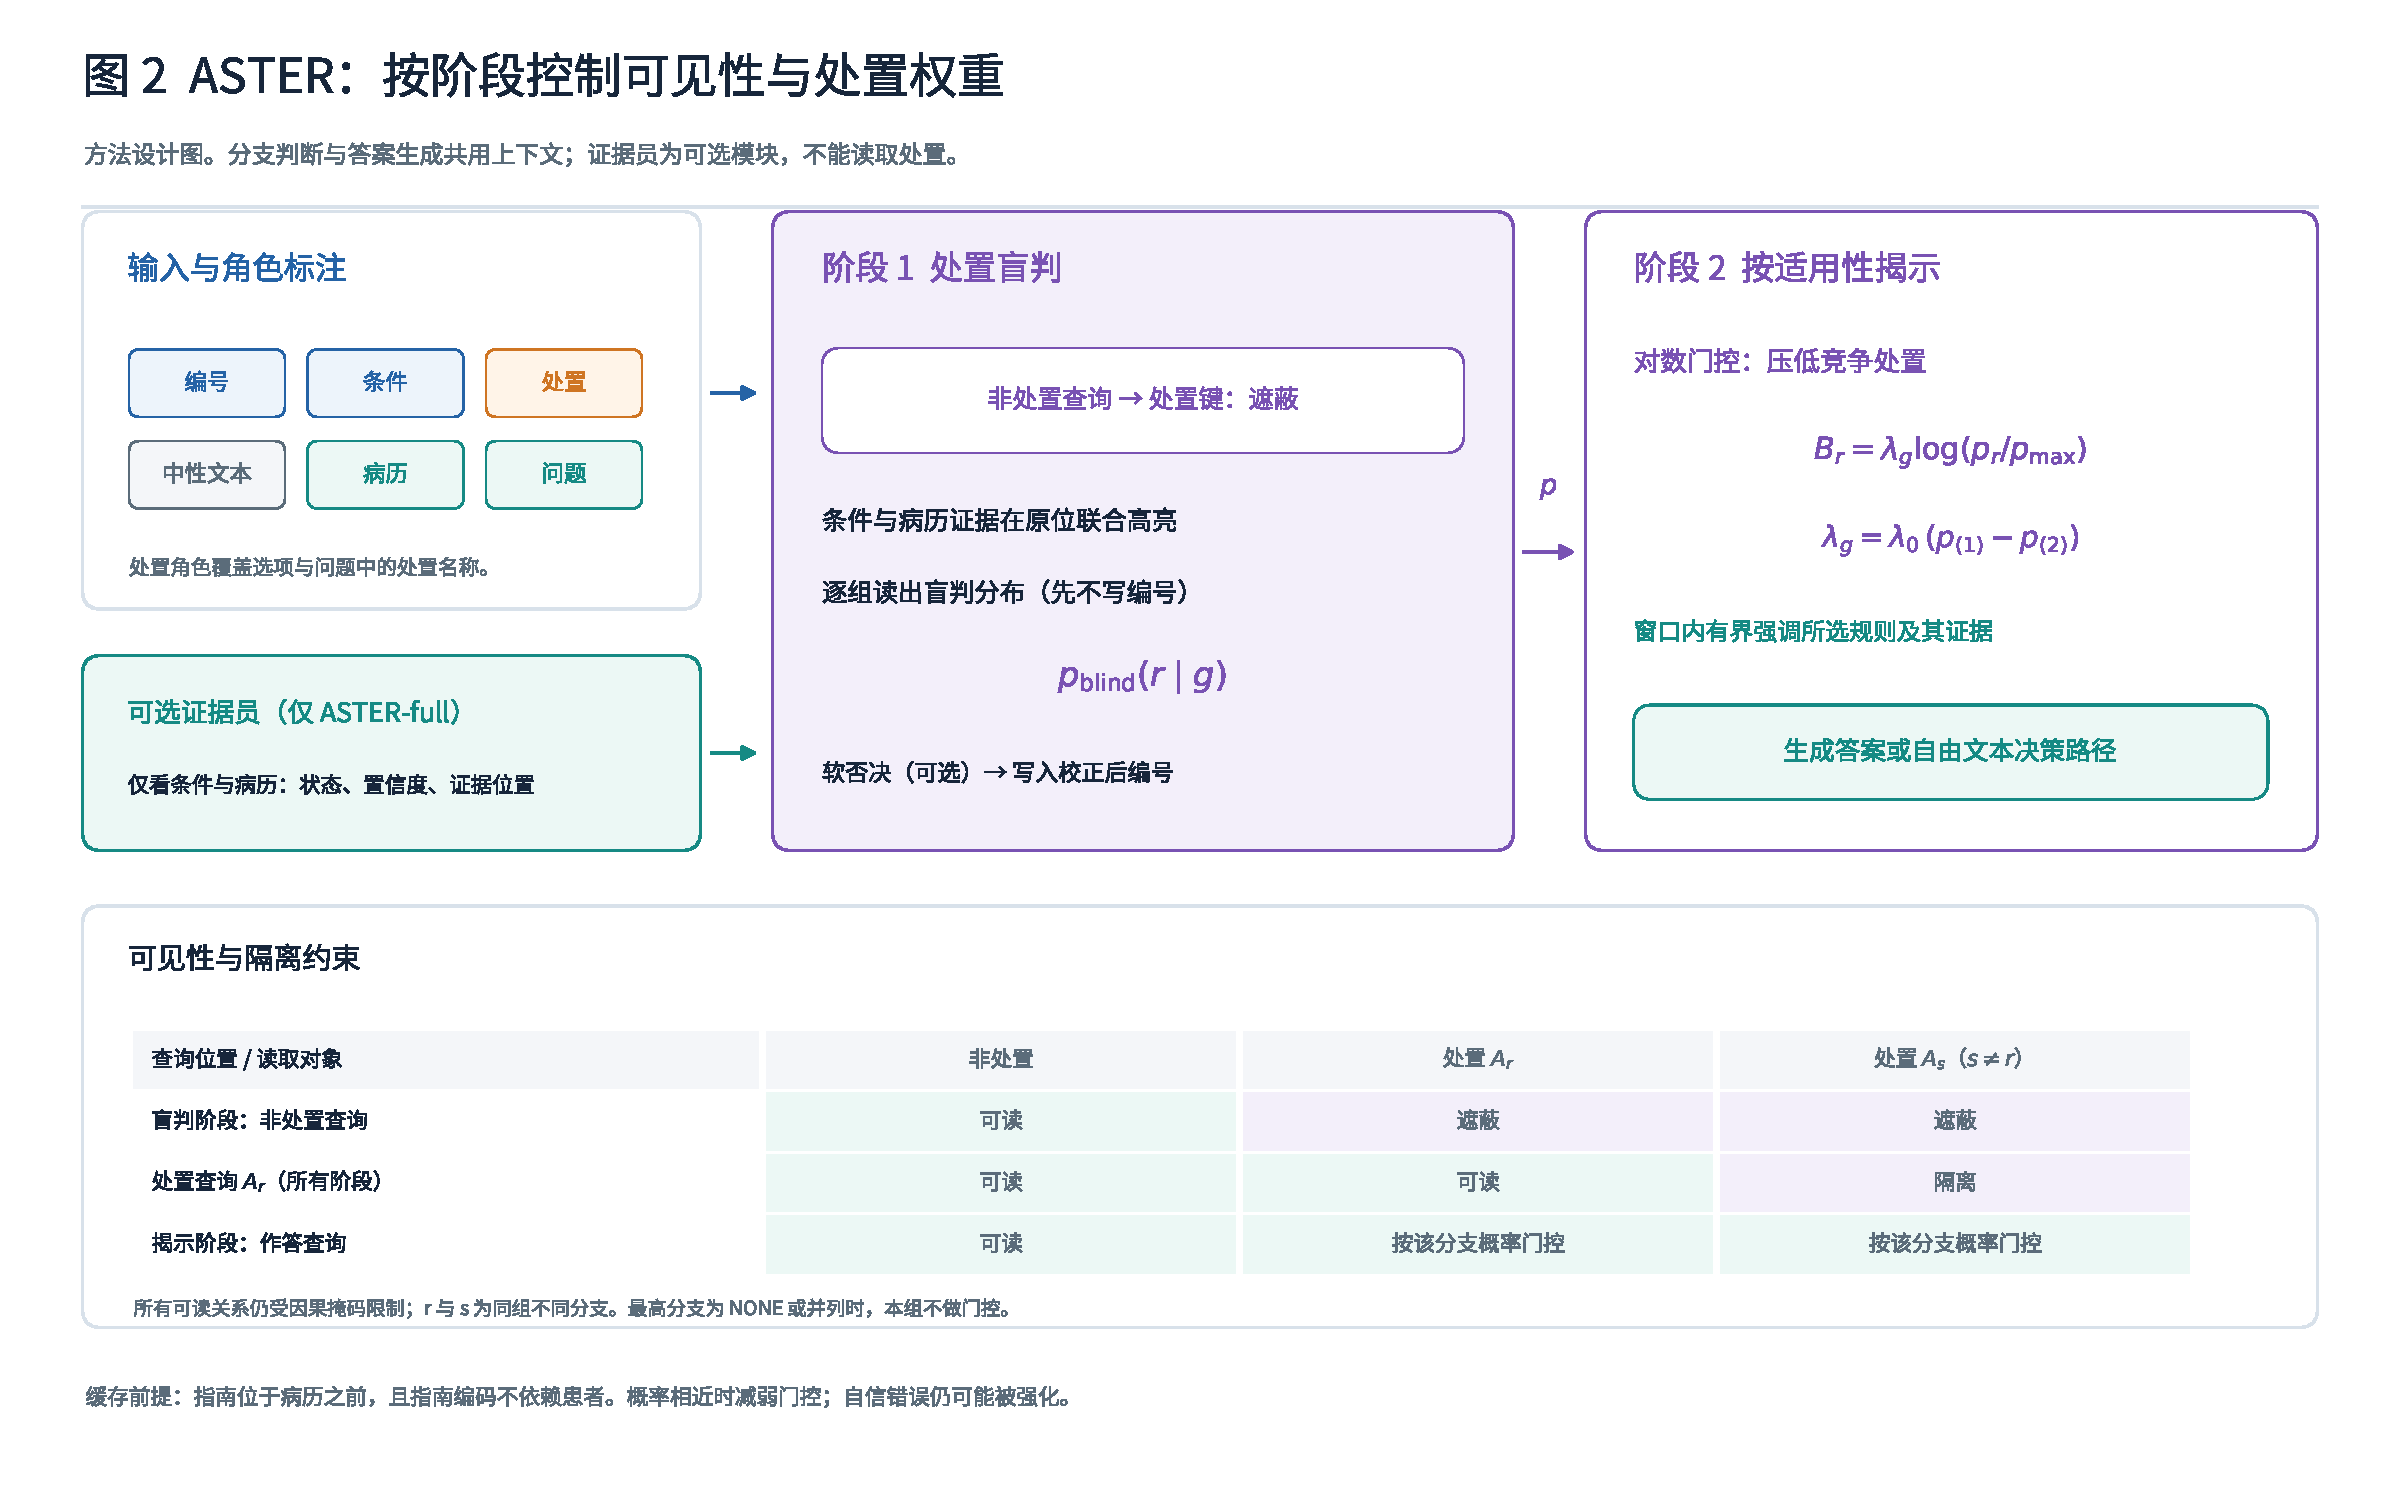
\includegraphics[width=\textwidth]{fig02_aster.pdf}
  \caption{\textbf{ASTER operators in a shared full context.} (a) The matrix shows representative-token query-key masks combined with causal masking. All BLIND non-action queries, including omitted neutral N and question Q positions, are blocked from action keys. Action mentions in questions/options retain the act role. The black outline marks cross-fragment action isolation, maintained in both phases. B is a fixed non-action readout position before branch-ID writing. (b) The optional clerk reads conditions C and patient text P and returns atomic states, confidence, and evidence. ASTER-full jointly highlights condition/evidence spans $(C,E)$ for post-prefix queries and applies a soft veto to obtain $p$ from $p_{\mathrm{blind}}$, both including NONE. This is joint highlighting, not pairwise binding. The adjusted distribution determines the written ID and both REVEAL controls. (c) For $p_1>\max(p_2,p_{\mathrm{NONE}})$, gating adds $b_r=\lambda_g\log(p_r/p_{\max})$ to rule-action keys across all layers/heads; emphasis adds bounded $\beta$ to selected rule/evidence tokens within specified layers when $p_{\max}\ge\tau$. Ties or a top NONE disable both controls. Purple elements are ASTER-full only. Only a fixed, patient-independent guideline prefix is cached; patient-dependent operations follow it.}
  \label{fig:aster-method}
\end{figure*}

\begin{figure*}[t]
  \centering
  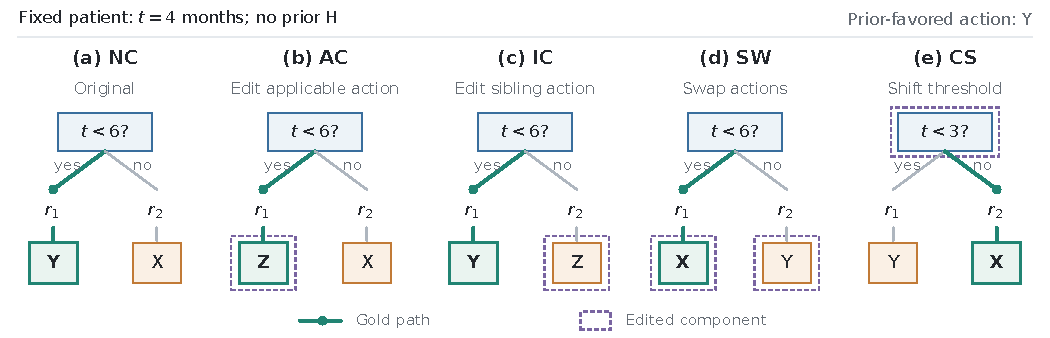
\includegraphics[width=\textwidth]{fig03_protocol.pdf}
  \caption{\textbf{Five paired guideline variants for a fixed fictional patient.} Each panel uses $t=4$ months and no prior H. NC retains the original rules; AC replaces the applicable action; IC replaces only the sibling action; SW exchanges the two actions; and CS shifts the threshold from 6 to 3 months, changing the applicable branch. The gold routes are $r_1\to Y$, $r_1\to Z$, $r_1\to Y$, $r_1\to X$, and $r_2\to X$, respectively. Identical tree layouts expose the local intervention: dashed outlines mark edited components, and the emphasized path marks the gold route. The common no-H condition is omitted from the miniature trees. Y is stipulated to be prior-favored in this illustration. SW reproduces the task in Figure 1; no model predictions are shown.}
  \label{fig:aster-protocol}
\end{figure*}

\begin{figure*}[t]
  \centering
  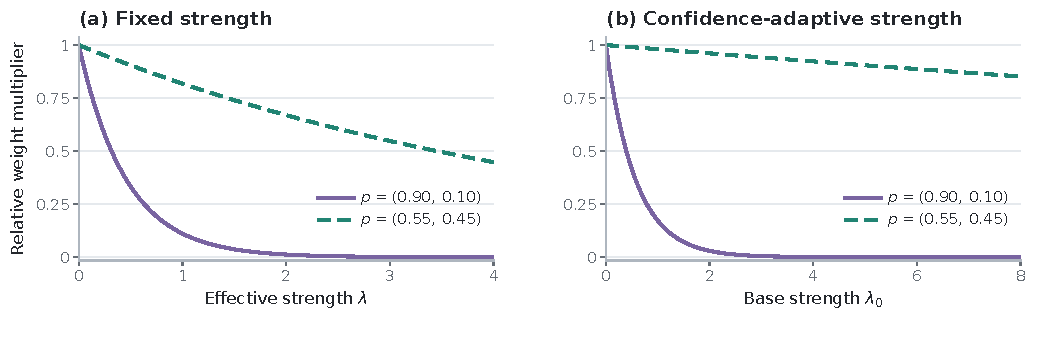
\includegraphics[width=\textwidth]{fig04_gate.pdf}
  \caption{\textbf{Analytic effect of the logarithmic action gate.} For fixed branch probabilities, pre-gate attention scores, and other biases, the gate multiplies the competing-to-top action-weight ratio by $m=(p_{\mathrm{comp}}/p_{\mathrm{top}})^\lambda$. (a) The effective strength $\lambda$ is varied directly. (b) The base strength $\lambda_0$ is varied with $\lambda=\lambda_0(p_{\mathrm{top}}-p_{\mathrm{comp}})$. Curves use the declared two-rule distributions $(0.90,0.10)$ and $(0.55,0.45)$, with zero NONE mass. They are exact formula evaluations, not measured attention probabilities, accuracy, or robustness. The plotted quantity is a relative multiplier on unnormalized attention weight, rather than the selected branch's share of total attention.}
  \label{fig:aster-gate}
\end{figure*}


% Paths are relative to the LaTeX compilation directory. If compiling from a
% paper/ subdirectory, use ../docs/ASTER/figures/ in both paths instead.
% Each source PDF is 7.0 inches wide. The template's \textwidth determines the
% final scale; inspect text at that scale in the final manuscript PDF.
% The English captions are mirrored in captions.en.md.

\begin{figure*}[t]
  \centering
  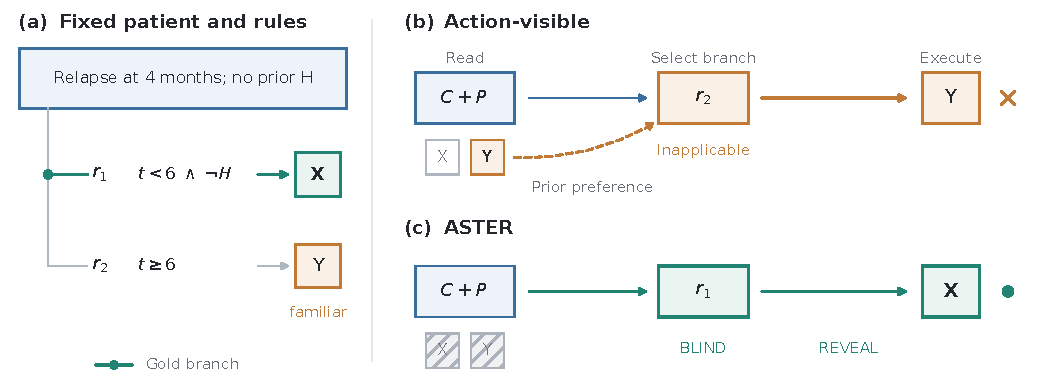
\includegraphics[width=\textwidth]{fig01_tlbs.pdf}
  \caption{\textbf{Treatment-led branch selection as a testable failure mode.} (a) In this fictional action-swap (SW) example, the patient relapses at $t=4$ months with no prior H. The supplied rules make $r_1:(t<6\land\neg H)\to X$ applicable and $r_2:(t\ge6)\to Y$ inapplicable. (b) The action-visible route illustrates the hypothesis that a preference for familiar Y can redirect selection toward its sibling branch. (c) ASTER is designed to select $r_1$ before revealing X. Both routes retain the same patient facts, conditions, and X/Y tokens; only the selection-stage attention mask changes. The dashed arrow and displayed outcomes are schematic, not observed model traces.}
  \label{fig:aster-tlbs}
\end{figure*}

\begin{figure*}[t]
  \centering
  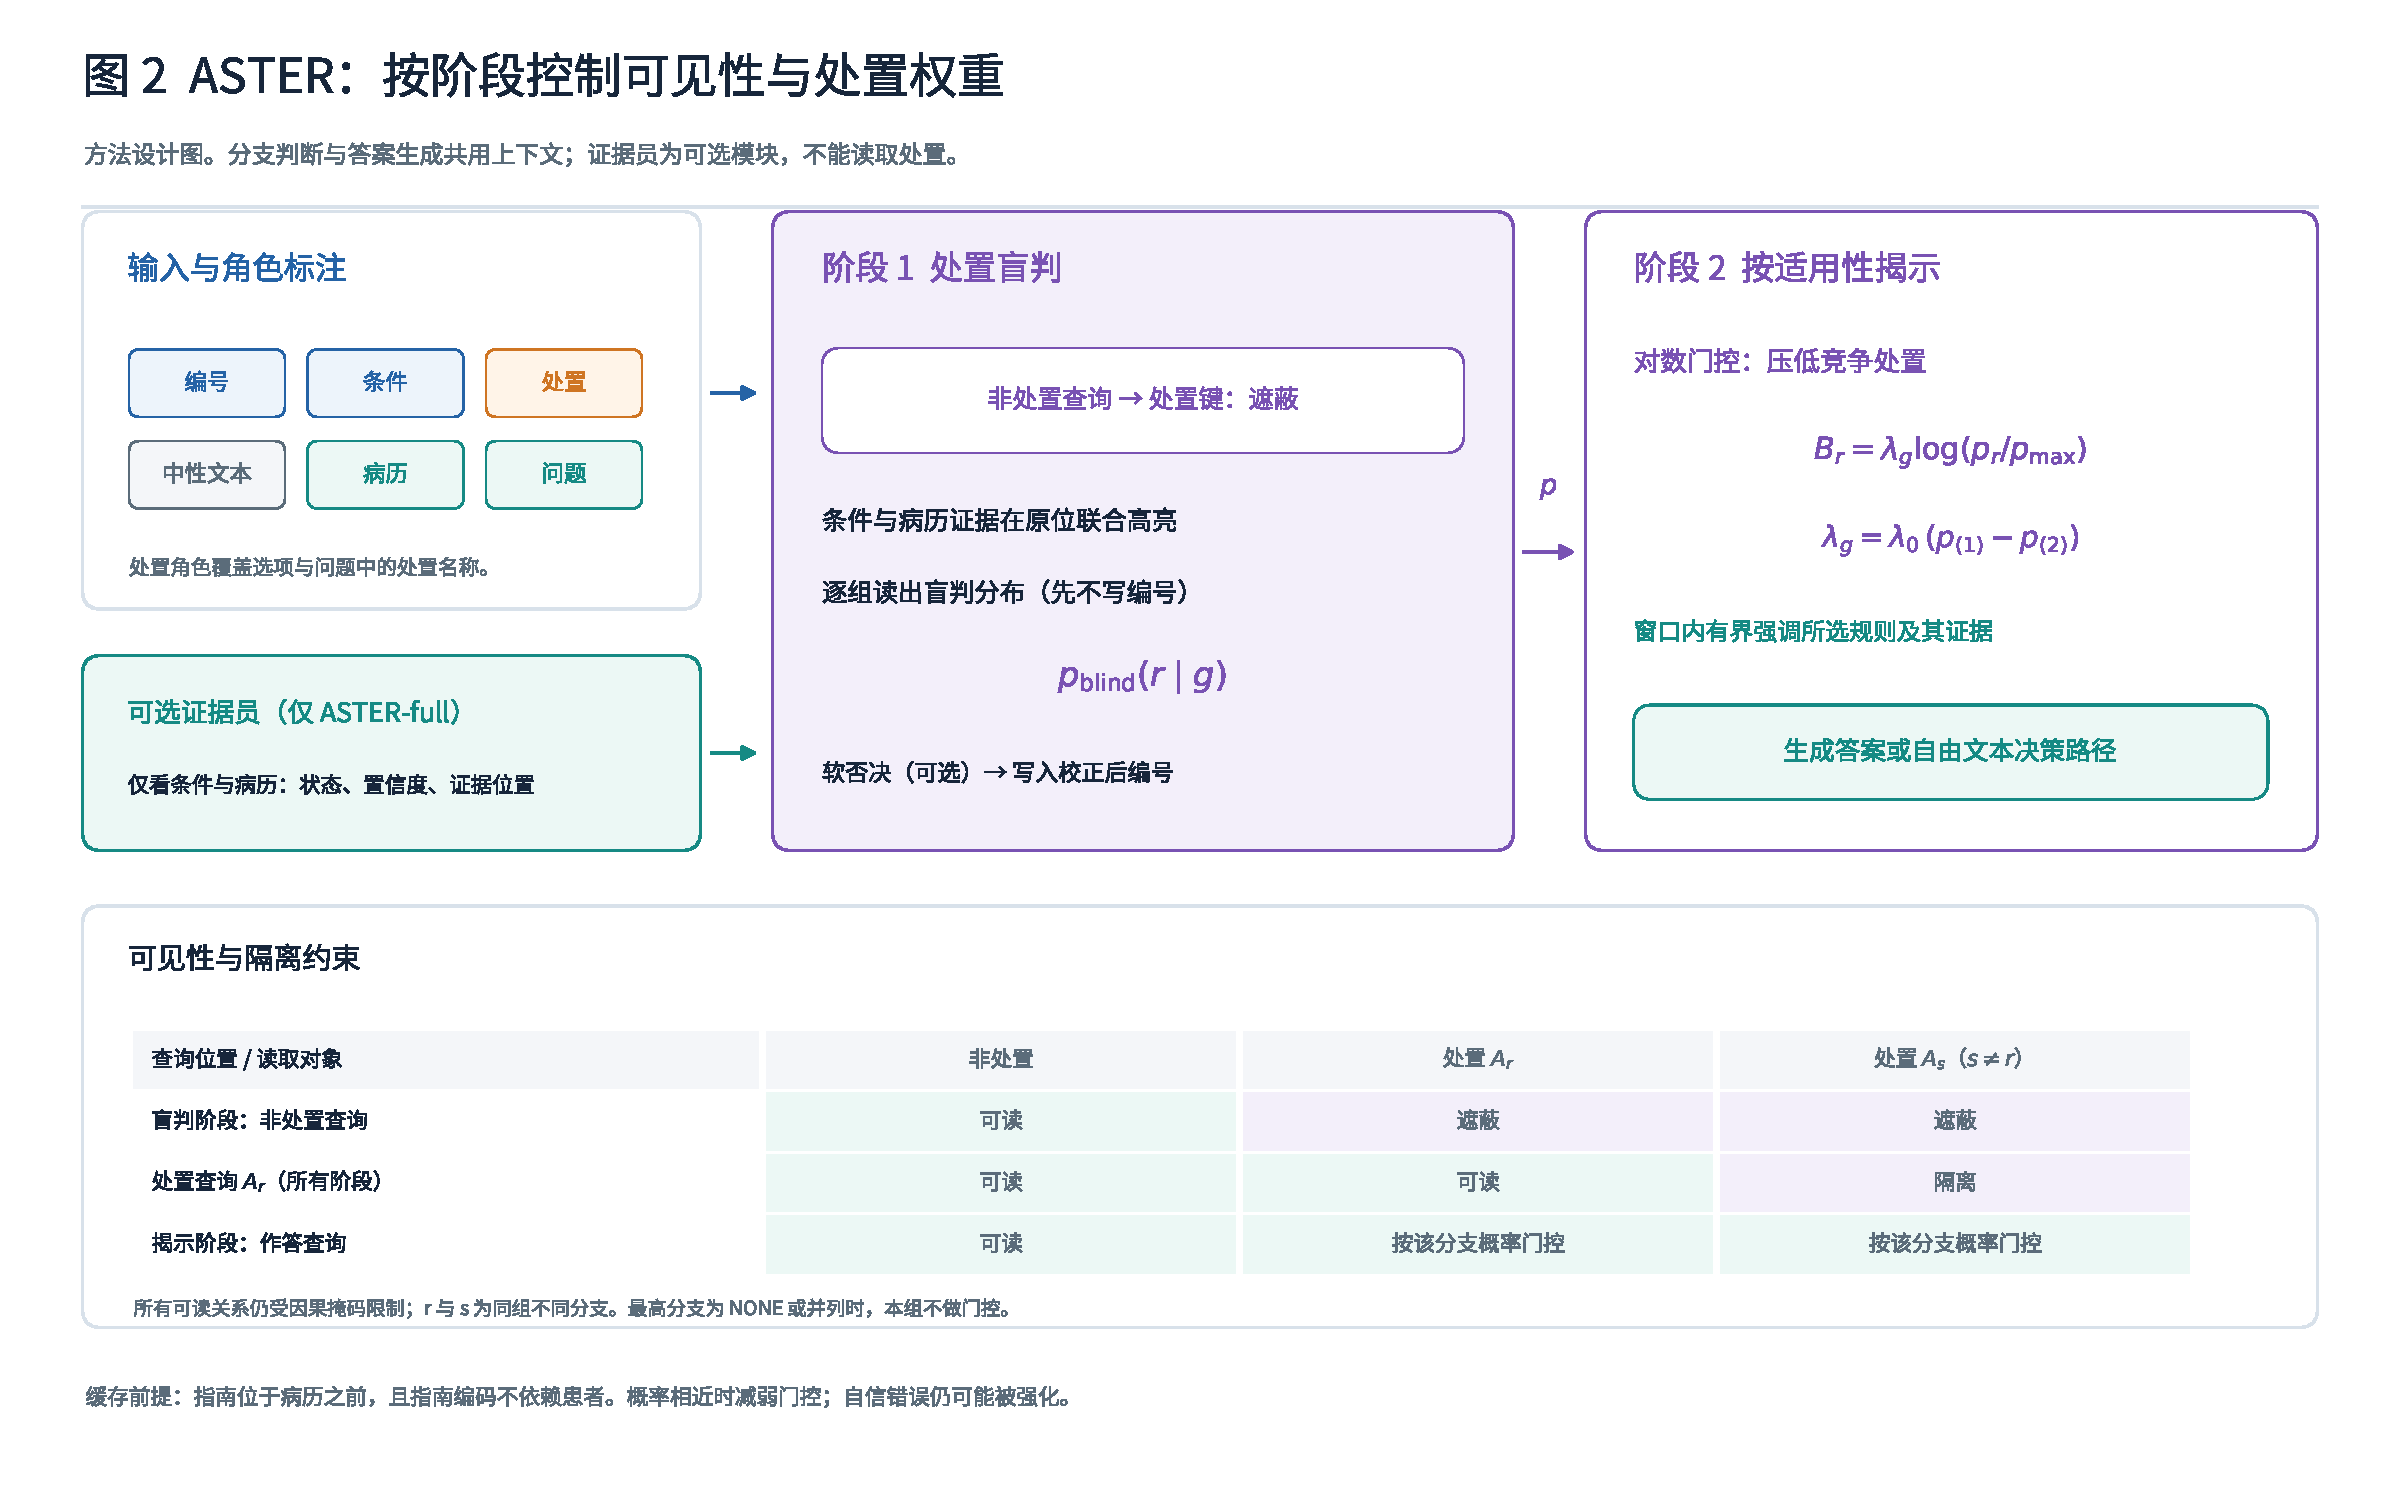
\includegraphics[width=\textwidth]{fig02_aster.pdf}
  \caption{\textbf{ASTER operators in a shared full context.} (a) The matrix shows representative-token query-key masks combined with causal masking. All BLIND non-action queries, including omitted neutral N and question Q positions, are blocked from action keys. Action mentions in questions/options retain the act role. The black outline marks cross-fragment action isolation, maintained in both phases. B is a fixed non-action readout position before branch-ID writing. (b) The optional clerk reads conditions C and patient text P and returns atomic states, confidence, and evidence. ASTER-full jointly highlights condition/evidence spans $(C,E)$ for post-prefix queries and applies a soft veto to obtain $p$ from $p_{\mathrm{blind}}$, both including NONE. This is joint highlighting, not pairwise binding. The adjusted distribution determines the written ID and both REVEAL controls. (c) For $p_1>\max(p_2,p_{\mathrm{NONE}})$, gating adds $b_r=\lambda_g\log(p_r/p_{\max})$ to rule-action keys across all layers/heads; emphasis adds bounded $\beta$ to selected rule/evidence tokens within specified layers when $p_{\max}\ge\tau$. Ties or a top NONE disable both controls. Purple elements are ASTER-full only. Only a fixed, patient-independent guideline prefix is cached; patient-dependent operations follow it.}
  \label{fig:aster-method}
\end{figure*}

\begin{figure*}[t]
  \centering
  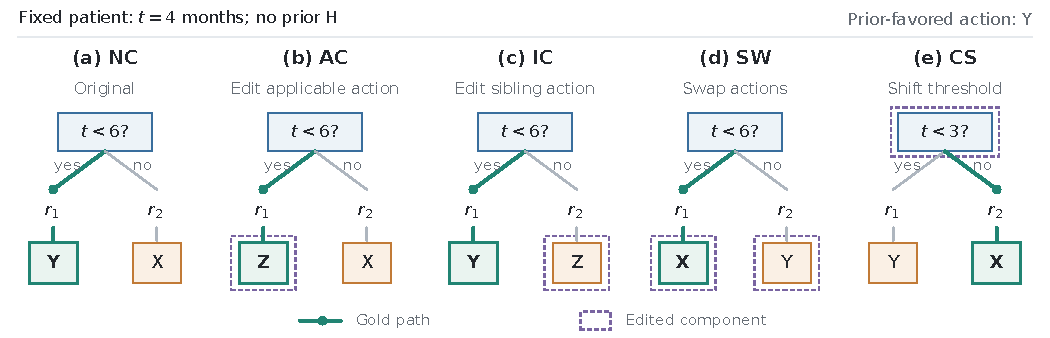
\includegraphics[width=\textwidth]{fig03_protocol.pdf}
  \caption{\textbf{Five paired guideline variants for a fixed fictional patient.} Each panel uses $t=4$ months and no prior H. NC retains the original rules; AC replaces the applicable action; IC replaces only the sibling action; SW exchanges the two actions; and CS shifts the threshold from 6 to 3 months, changing the applicable branch. The gold routes are $r_1\to Y$, $r_1\to Z$, $r_1\to Y$, $r_1\to X$, and $r_2\to X$, respectively. Identical tree layouts expose the local intervention: dashed outlines mark edited components, and the emphasized path marks the gold route. The common no-H condition is omitted from the miniature trees. Y is stipulated to be prior-favored in this illustration. SW reproduces the task in Figure 1; no model predictions are shown.}
  \label{fig:aster-protocol}
\end{figure*}

\begin{figure*}[t]
  \centering
  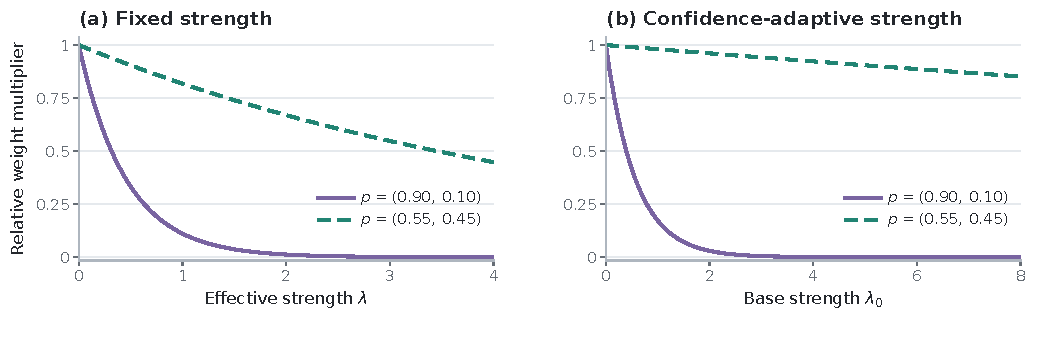
\includegraphics[width=\textwidth]{fig04_gate.pdf}
  \caption{\textbf{Analytic effect of the logarithmic action gate.} For fixed branch probabilities, pre-gate attention scores, and other biases, the gate multiplies the competing-to-top action-weight ratio by $m=(p_{\mathrm{comp}}/p_{\mathrm{top}})^\lambda$. (a) The effective strength $\lambda$ is varied directly. (b) The base strength $\lambda_0$ is varied with $\lambda=\lambda_0(p_{\mathrm{top}}-p_{\mathrm{comp}})$. Curves use the declared two-rule distributions $(0.90,0.10)$ and $(0.55,0.45)$, with zero NONE mass. They are exact formula evaluations, not measured attention probabilities, accuracy, or robustness. The plotted quantity is a relative multiplier on unnormalized attention weight, rather than the selected branch's share of total attention.}
  \label{fig:aster-gate}
\end{figure*}

